\documentclass[11pt]{article}

%\usepackage{palatino}

\usepackage[utf8]{inputenc}
\usepackage[T1]{fontenc}
% Chivo como en las diapositivas o Fira Sans?
%\usepackage[familydefault,regular]{Chivo}
\usepackage[sfdefault,scaled=.85]{FiraSans}
\usepackage{newtxsf}
\usepackage{mathastext}
\usepackage[spanish]{babel}
\setlength{\parindent}{0pt}
\usepackage{amssymb}
\usepackage{amsmath}
\usepackage{wasysym}
\usepackage[x11names, rgb, html]{xcolor}
\usepackage{graphics}
\usepackage{caption}
\usepackage{lipsum}
\usepackage{float}
\usepackage{adjustbox}
\usepackage{geometry}
\usepackage[scaled=.85]{FiraMono}
\usepackage{algpseudocode}
\usepackage{algorithm}
\usepackage{hyperref}

\hypersetup{
  % hidelinks = true,   % Oculta todos los enlaces.
  colorlinks = true,   % Muestra todos los enlaces, sin bordes alrededor.
  linkcolor={black},     % Color de enlaces genéricos
  citecolor={black},   % Color de enlaces de referencias
  urlcolor={blue!70!black}     % Color de enlaces de URL
}

\geometry{left=3cm,right=3cm,top=3cm,bottom=3cm,headheight=1cm,headsep=0.5cm}

%%% PGFPLOTSTABLE

\usepackage{pgfplotstable}

%%% COLORES

\definecolor{50}{HTML}{FFEBEE}
\definecolor{100}{HTML}{FFCDD2}
\definecolor{200}{HTML}{EF9A9A}
\definecolor{300}{HTML}{E57373}
\definecolor{400}{HTML}{EF5350}
\definecolor{500}{HTML}{F44336}
\definecolor{600}{HTML}{E53935}
\definecolor{700}{HTML}{D32F2F}
\definecolor{800}{HTML}{C62828}
\definecolor{900}{HTML}{B71C1C}



%% Colores de Solarized

\definecolor{sbase03}{HTML}{002B36}
\definecolor{sbase02}{HTML}{073642}
\definecolor{sbase01}{HTML}{586E75}
\definecolor{sbase00}{HTML}{657B83}
\definecolor{sbase0}{HTML}{839496}
\definecolor{sbase1}{HTML}{93A1A1}
\definecolor{sbase2}{HTML}{EEE8D5}
\definecolor{sbase3}{HTML}{FDF6E3}
\definecolor{syellow}{HTML}{B58900}
\definecolor{sorange}{HTML}{CB4B16}
\definecolor{sred}{HTML}{DC322F}
\definecolor{smagenta}{HTML}{D33682}
\definecolor{sviolet}{HTML}{6C71C4}
\definecolor{sblue}{HTML}{268BD2}
\definecolor{scyan}{HTML}{2AA198}
\definecolor{sgreen}{HTML}{859900}

%% Colores del documento

\definecolor{text}{RGB}{78,78,78}
\definecolor{accent}{RGB}{129, 26, 24}

%%% LISTINGS

\usepackage{listingsutf8}

%% Las tildes

\lstset{
  inputencoding=utf8/latin1
}

%% Colores de Solarized para listings

\lstset{
  % How/what to match
  % sensitive=true,
  % language=pseudo,
  % Border (above and below)
  frame=leftline,
  rulecolor=\color{300},
  framerule=2pt,
  % Line number
  numbers=left,
  % Extra margin on line (align with paragraph)
  xleftmargin=\parindent,
  % Put extra space under caption
  belowcaptionskip=1\baselineskip,
  % Colors
  % backgroundcolor=\color{sbase3},
  basicstyle=\footnotesize\ttfamily\color{sbase00},
  keywordstyle=\color{700},
  commentstyle=\color{300},
  stringstyle=\color{500},
  numberstyle=\color{500},
  %identifierstyle=\color{500},
  % Break long lines into multiple lines?
  breaklines=true,
  % Show a character for spaces?
  showstringspaces=false,
  tabsize=2,
  xleftmargin=0.7em,
}

\renewcommand{\lstlistingname}{Código fuente}% Listing -> Algorithm

%%% INFORMACIÓN DEL DOCUMENTO

\title{Fundamentos de Redes\\ \Large{Definición e implementación de un protocolo de aplicación}}
\author{José María Martín Luque\\ Antonio Coín Castro\\ \vspace{.5em}Grupo 2}
\begin{document}


\maketitle

\section{Descripción de la aplicación: conversor de imágenes}

Vamos a programar una aplicación, siguiendo el paradigma \textit{cliente/servidor}, que sirva como conversor de imágenes de formato JPEG a PNG y viceversa.\\

En nuestro modelo, el cliente actúa como un usuario que posee una imagen en un formato concreto, y quiere convertirla al otro. El servidor, por su parte, actúa como un conversor, que aporta la funcionalidad necesaria para modificar el formato de la imagen y devolverla al cliente.\\

Utilizaremos sockets TCP como medio de comunicación entre el cliente y el servidor, pues al tratarse de una imagen, no podemos permitir que se pierdan datos en el proceso, que lleguen desordenados, etc. Además, el servidor procesará las peticiones de varios clientes de forma \textbf{concurrente}.\\

A grandes rasgos, el funcionamiento es el siguiente: el cliente establece una conexión con 
el servidor, que le proporciona un menú donde elegir el formato de conversión. Una vez elegido, el cliente envía por el canal TCP la imagen como una cadena de bytes, y el servidor la recibe, la procesa, y la devuelve de nuevo como una cadena de bytes, ya en el formato correcto.\\

El lenguaje elegido para programar la aplicación es \textbf{Go}. Hemos elegido este lenguaje por su facilidad de gestión de servicios en red, así como la simplicidad con la que gestiona la concurrencia (mediante las llamadas \textit{goroutines}). Empleamos una librería de conversión de imágenes para aportar la funcionalidad deseada.
\newpage 
\section{Diagrama de estados del servidor}

Mostramos ahora un diagrama de los posibles estados en los que puede encontrarse el servidor al establecer conexión con un cliente.
\begin{center}
	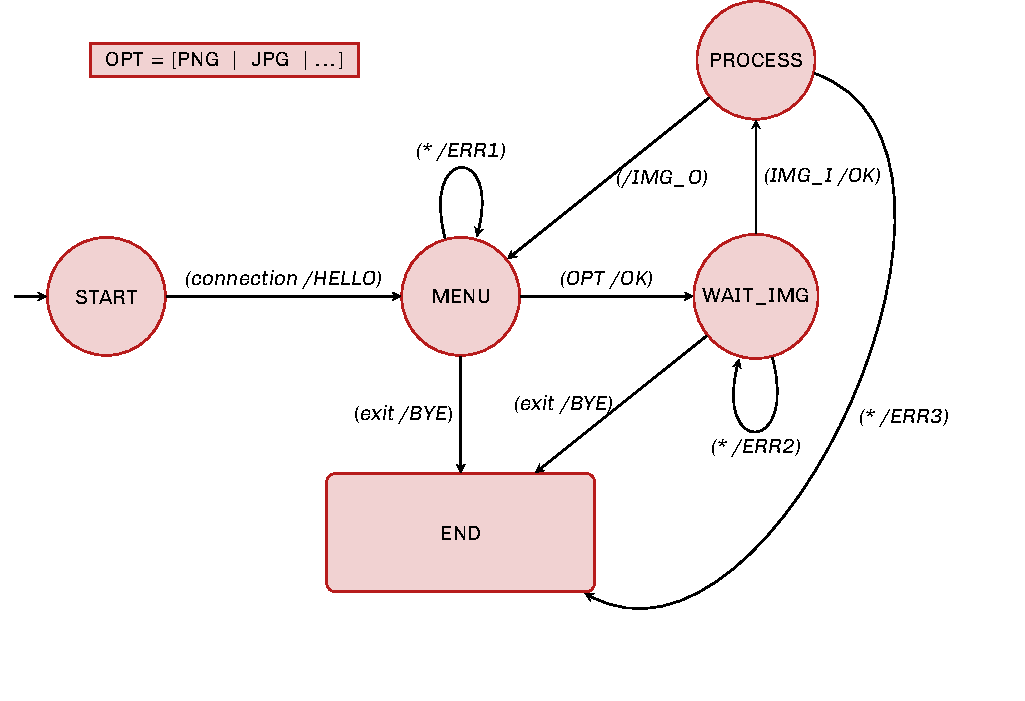
\includegraphics[width=.9\textwidth]{img/diagrama}
\end{center}	


\section{Mensajes que intervienen}

Los distintos mensajes que intervienen en la comunicación son los siguientes. Los errores se manejan de forma apropiada dentro de los programas del cliente y del servidor.

\subsection{Cliente}
\begin{center}
	\begin{tabular}{|c|c|c|}
	\hline
	Código & Cuerpo & Descripción\\
	\hline
	00 & OPT + o & Opción de formato a convertir: o\\
	\hline
	01 & IMG\_I + img & Datos de la imagen a convertir: img\\
	\hline
\end{tabular}
\end{center}


\subsection{Servidor}
\begin{center}
	\begin{tabular}{|c|c|c|}
	\hline
	Código & Cuerpo & Descripción\\
	\hline
	10 & HELLO & Conexión establecida\\
	\hline
	11 & OK & Datos recibidos correctamente\\
	\hline
	12 & ERR1 + str & Opción incorrecta\\
	\hline
	13 & ERR2 + str & Fallo al recibir la imagen\\
	\hline
	14 & ERR3 + str & Fallo al procesar la imagen\\
	\hline
	15 & IMG\_O + img & Imagen convertida: img\\
	\hline
	16 & BYE & Finalizar la conexión\\
	\hline 
\end{tabular}	
\end{center}

\section{Evaluación de la aplicación}

Por último, mostramos evidencia gráfica de que la aplicación funciona correctamente.

\begin{figure}[h]
	\centering
	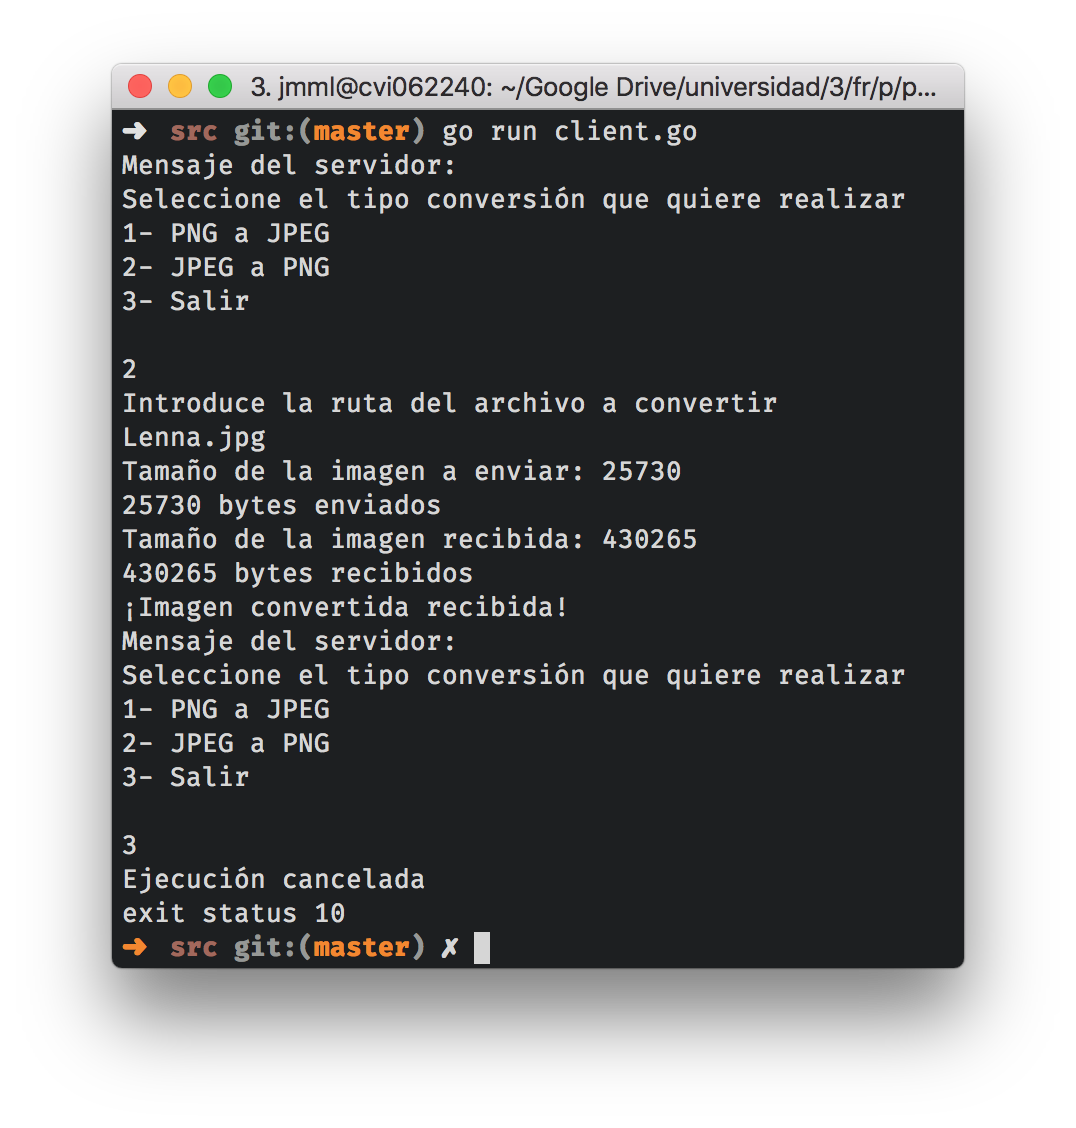
\includegraphics[width=.5\textwidth]{img/cliente}
	\caption{Ejemplo de ejecución de un cliente}
\end{figure}

Como vemos, el cliente selecciona la opción del menú que desee, y a continuación especifica la ruta donde se encuentra la imagen a convertir. La imagen convertida se envía de vuelta al cliente por el canal TCP, y este la guarda en el directorio donde se encontraba la imagen original.

\begin{figure}[ht!]
	\centering
	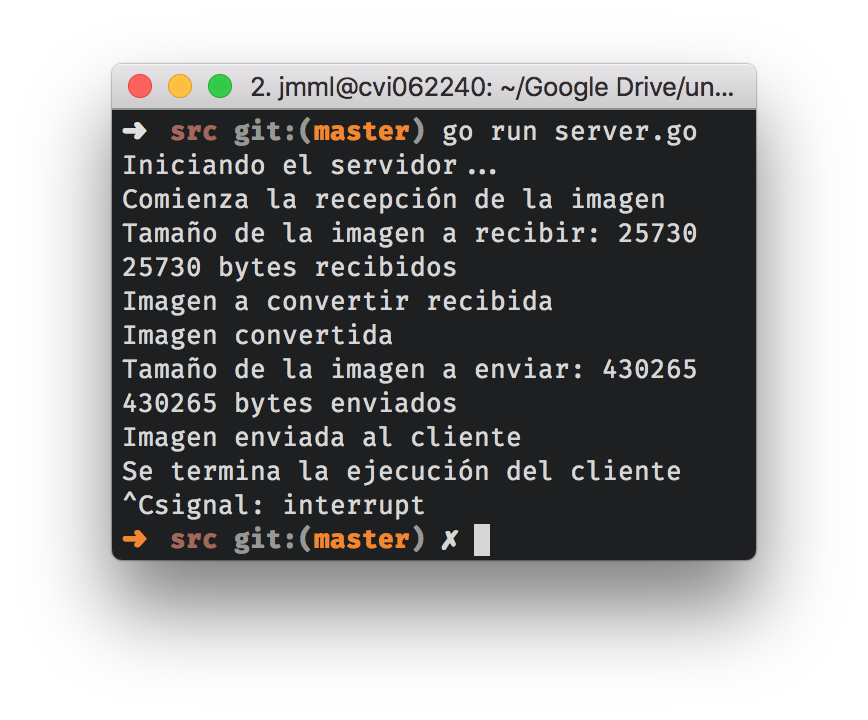
\includegraphics[width=.5\textwidth]{img/servidor}
	\caption{Ejemplo de ejecución del servidor}
\end{figure}

Cuando el servidor detecta la conexión de algún cliente, envía el menú para que este pueda elegir el formato, y a continuación espera la recepción de la imagen. Una vez recibida, la procesa para convertirla y la devuelve, quedando a la espera de dar servicio a más clientes.
	
\end{document}
